%!TEX root = ../../book_ML.tex

\setcounter{chapter}{-1}
\chapter{Lời nói đầu}
\label{cha:introduce}

Những năm gần đây, \textbf{\textit{trí tuệ nhân tạo}} ({artificial
intelligence, AI}) dần nổi lên như một minh chứng cho cuộc cách mạng công
nghiệp lần thứ tư, sau động cơ hơi nước, năng lượng điện và công nghệ thông
tin. Trí tuệ nhân tạo đã và đang trở thành nhân tố cốt lõi trong các hệ thống
công nghệ cao. Thậm chí, nó đã len lỏi vào hầu hết các lĩnh vực của đời sống mà
có thể chúng ta không nhận ra. Xe tự hành của Google và Tesla, hệ thống tự tag
khuôn mặt trong ảnh của Facebook, trợ lý ảo Siri của Apple, hệ thống gợi ý sản
phẩm của Amazon, hệ thống gợi ý phim của Netflix, hệ thống dịch đa ngôn ngữ
Google Translate, máy chơi cờ vây AlphaGo và gần đây là AlphaGo Zero của Google
DeepMind,... chỉ là một vài ứng dụng nổi bật trong vô vàn những ứng dụng của
trí tuệ nhân tạo.

\textbf{\textit{Học máy}} ({machine learning, ML}) là một tập con của
trí tuệ nhân tạo. Machine learning là một lĩnh vực nhỏ trong khoa học máy tính,
có khả năng tự học hỏi dựa trên dữ liệu được đưa vào mà không cần phải được lập
trình cụ thể (\textit{Machine Learning is the subfiled of computer science, that
``gives computers the ability to learn without being explicitly programmed''} --
Wikipedia).

Những năm gần đây, sự phát triển của các hệ thống tính toán cùng lượng dữ liệu
khổng lồ được thu thập bởi các hãng công nghệ lớn đã giúp machine learning tiến
thêm một bước dài. Một lĩnh vực mới được ra đời được gọi là \textbf{\textit{học
sâu}} ({deep learning, DL}). Deep learning đã giúp máy tính thực thi
những việc vào mười năm trước tưởng chừng là không thể: phân loại cả ngàn vật
thể khác nhau trong các bức ảnh, tự tạo chú thích cho ảnh, bắt chước giọng nói
và chữ viết, giao tiếp với con người, chuyển đổi ngôn ngữ, hay thậm chí cả sáng
tác văn thơ và âm nhạc\footnote{Đọc thêm: \textit{8 Inspirational Applications
of Deep Learning} (\url{https://goo.gl/Ds3rRy}).}.

% Bạn đọc cần phân biệt rõ ba khái niệm \textit{artificial intelligence, machine
% learning}, và \textit{deep learning}\footnote{Đọc thêm:
% \textit{What’s the Difference Between Artificial Intelligence, Machine
% Learning, and Deep Learning?} (\url{https://goo.gl/NNwGCi})}.

% Mối quan hệ giữa artificial intelligence, machine learning, và deep learning
% được minh hoạ trong Hình~\ref{fig:0_1}.
%% *****************************************************************************
\begin{figure}[]
\centering
    % 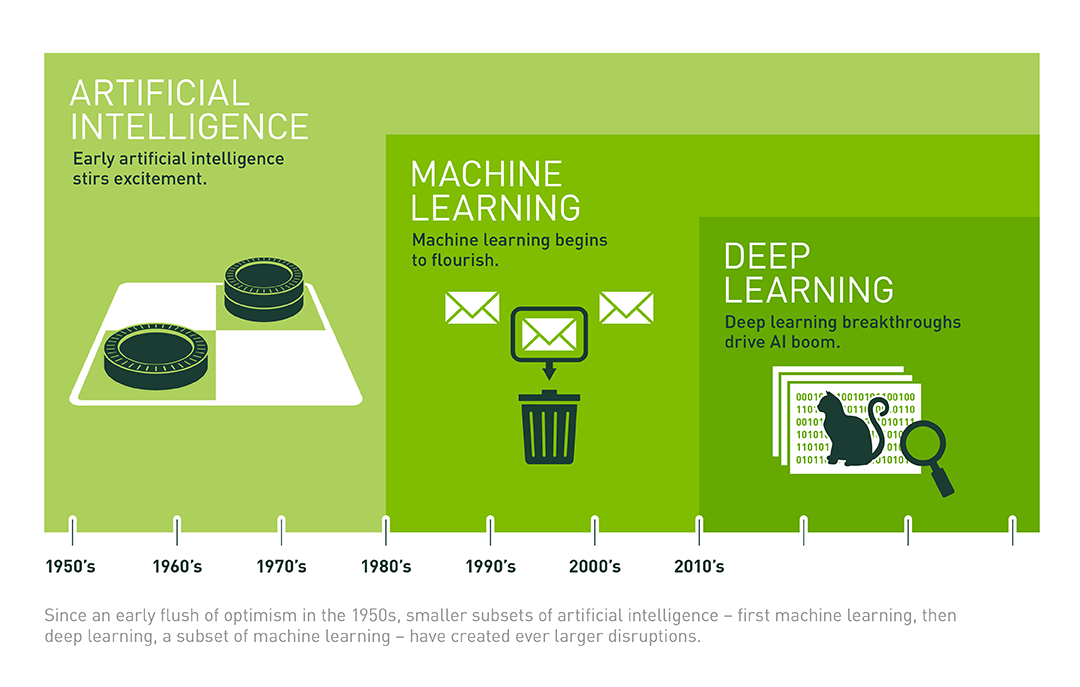
\includegraphics[width = \textwidth]{Chapters/00_loinoidau/dl.png}
    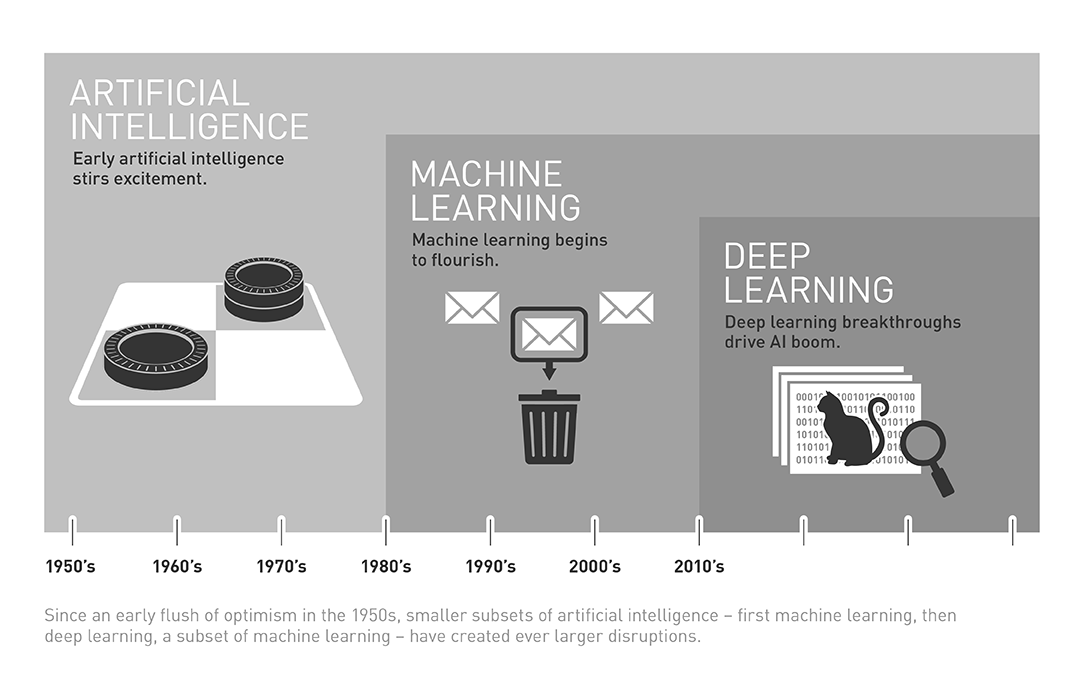
\includegraphics[width = .9\textwidth]{Chapters/00_loinoidau/dl_gray.png}
    \caption[]{Mối quan hệ giữa AI, ML, và DL. (Nguồn \textit{What’s the Difference Between Artificial
    Intelligence, Machine Learning, and Deep Learning?} --
    \url{https://goo.gl/NNwGCi}).}
    \label{fig:0_1}
\end{figure}
%% *****************************************************************************
\newnote{Mối quan hệ AI-ML-DL}{ DL là một tập con của ML. ML là một tập con của
AI (xem Hình~\ref{fig:0_1}). }

\section{Mục đích của cuốn sách}
Những phát triển thần kỳ của trí tuệ nhân tạo dẫn tới nhu cầu cao về mặt nhần
lực làm việc trong các ngành liên quan tới machine learning ở Việt Nam cũng như
trên thế giới. Đó cũng là nguồn động lực để tác giả gây dựng và phát triển
blog Machine Learning cơ bản từ đầu năm 2017
(\url{https://machinelearningcoban.com}). Tính tới thời điểm đặt bút viết những
dòng này, blog đã có hơn một triệu lượt ghé thăm. Facebook page Machine Learning
cơ bản\footnote{\url{https://goo.gl/wyUEjr}} chạm mốc 14 nghìn lượt likes, Forum
Machine Learning cơ bản\footnote{\url{https://goo.gl/gDPTKX}} đạt tới 17 nghìn
thành viên. Trong quá trình viết blog và duy trì các trang Facebook, tác giả đã
nhận được nhiều sự ủng hộ của bạn đọc về tinh thần cũng như vật chất. Nhiều
bạn đọc cũng khuyến khích tác giả tổng hợp kiến thức trên blog thành một
cuốn sách cho cộng đồng những người tiếp cận với ML bằng tiếng
Việt. Sự ủng hộ và những lời động viên đó là động lực lớn cho tác giả khi bắt
tay vào thực hiện và hoàn thành cuốn sách này.


Lĩnh vực ML nói chung và DL nói riêng là cực kỳ lớn và có nhiều nhánh nhỏ. Phạm vi
một cuốn sách chắc chắn không thể bao quát hết mọi vấn đề và đi sâu vào từng
nhánh cụ thể. Do vậy, cuốn sách này chỉ nhằm cung cấp cho bạn đọc những
khái niệm, kỹ thuật chung và các thuật toán cơ bản nhất của ML. Từ đó, bạn đọc
có thể tự tìm thêm các cuốn sách và khóa học liên quan nếu muốn đi sâu vào từng
vấn đề.



Hãy nhớ rằng \textit{luôn bắt đầu từ những điều đơn giản}. Khi bắt tay vào giải
quyết một bài toán ML hay bất cứ bài toán nào, chúng ta nên bắt đầu từ những
thuật toán đơn giản. Không phải chỉ có những thuật toán phức tạp mới có thể
giải quyết được vấn đề. Những thuật toán phức tạp thường có yêu cầu cao về khả
năng tính toán và đôi khi nhạy cảm với cách chọn tham số. Ngược lại, những
thuật toán đơn giản giúp chúng ta nhanh chóng có một bộ khung cho mỗi bài
toán. Kết quả của các thuật toán đơn giản cũng mang lại cái nhìn sơ bộ về sự
phức tạp của mỗi bài toán. Việc cải thiện kết quả sẽ được thực hiện dần ở các
bước sau. Cuốn sách này sẽ trang bị cho bạn đọc những kiến thức khái quát và một
số hướng tiếp cận cơ bản cho các bài toán ML. Để tạo ra các sản phẩm thực tiễn,
chúng ta cần học hỏi và thực hành thêm nhiều.


\section{Hướng tiếp cận của cuốn sách}

Để giải quyết mỗi bài toán ML, chúng ta cần chọn một mô hình phù hợp. Mô hình
này được mô tả bởi bộ các tham số mà chúng ta cần đi tìm. Thông thường, lượng
tham số có thể lên tới hàng triệu và được tìm bằng cách giải một bài toán tối
ưu.

Khi viết về các thuật toán ML, tác giả sẽ bắt đầu từ những ý tưởng trực quan.
Những ý tưởng này được mô hình hoá dưới dạng một bài toán tối ưu. Các suy luận
toán học và ví dụ mẫu trên Python ở cuối mỗi chương sẽ giúp bạn đọc hiểu rõ hơn
về nguồn gốc, ý nghĩa, và cách sử dụng mỗi thuật toán. Xen kẽ giữa những thuật
toán ML, tác giả sẽ trình bày các kỹ thuật tối ưu cơ bản, với hy vọng giúp bạn
đọc hiểu rõ hơn bản chất của vấn đề.
%%%%%%%%%%%%%%%%
\section{Đối tượng của cuốn sách}
Cuốn sách được thực hiện hướng tới nhiều nhóm độc giả khác nhau. Nếu bạn không
thực sự muốn đi sâu vào phần toán, bạn vẫn có thể tham khảo mã nguồn và cách sử
dụng các thư viện. Nhưng để sử dụng các thư viện một cách hiệu quả, bạn cũng cần
hiểu nguồn gốc của mô hình và ý nghĩa của các tham số. Còn nếu bạn thực sự muốn
tìm hiểu nguồn gốc, ý nghĩa của các thuật toán, bạn có thể học được nhiều điều
từ cách xây dựng và tối ưu các mô hình. Phần tổng hợp các kiến thức toán cần
thiết trong Phần~\ref{part:math} sẽ là một nguồn tham khảo súc tích bất cứ khi
nào bạn có thắc mắc về các dẫn giải toán học. Phần~\ref{part:cvxopt} được dành
riêng để nói về tối ưu lồi -- một mảng quan trọng trong tối ưu, phù hợp với các
bạn thực sự muốn đi sâu thêm về tối ưu.

Các dẫn giải toán học được xây dựng phù hợp với chương trình toán phổ thông và
đại học ở Việt Nam. Các từ khóa khi được dịch sang tiếng Việt đều dựa trên những
tài liệu tác giả được học trong nhiều năm tại Việt Nam.

Phần cuối cùng của sách có mục Index các thuật ngữ quan trọng và thuật ngữ tiếng Anh đi kèm giúp bạn dần làm quen khi đọc các tài liệu tiếng Anh. 


\section{Yêu cầu về kiến thức}

Để có thể bắt đầu đọc cuốn sách này, bạn cần có một kiến thức nhất định về đại
số tuyến tính, giải tích ma trận, xác suất thống kê, và kỹ năng lập trình.

Phần~\ref{part:math} của cuốn sách ôn tập lại các kiến thức toán quan trọng được
dùng trong ML. Khi gặp khó khăn về toán, bạn được khuyến khích đọc lại các
chương trong phần này.

\index{numpy}
\index{scikit-learn}
\index{sklearn}
Ngôn ngữ lập trình được sử dụng trong cuốn sách là Python. Python là một ngôn
ngữ lập trình miễn phí, có thể được cài đặt dễ dàng trên các nền tảng hệ điều
hành khác nhau. Quan trọng hơn, có rất nhiều thư viện hỗ trợ ML cũng như DL
trên Python. Có hai thư viện Python chính thường được sử dụng trong
cuốn sách là numpy và scikit-learn. 

Numpy (\url{http://www.numpy.org/}) là một thư viện phổ biến giúp xử lý các phép
toán liên quan đến các mảng nhiều chiều, hỗ trợ các hàm gần gũi với đại số tuyến
tính. Nếu bạn đọc chưa quen thuộc với numpy, bạn có thể tham gia một khóa học
ngắn miễn phí trên trang web kèm theo cuốn sách này (\url{https://fundaml.com}).
Bạn sẽ được làm quen với cách xử lý các mảng nhiều chiều với nhiều ví dụ và bài
tập thực hành. Các kỹ thuật xử lý mảng trong cuốn sách này đều được đề cập tại
đây.

Scikit-learn, hay sklearn (\url{http://scikit-learn.org/}), là một thư viện chứa
đầy đủ các thuật toán ML cơ bản và rất dễ sử dụng. Tài liệu của scikit-learn
cũng là một nguồn tham khảo chất lượng cho các bạn làm ML. Scikit-learn sẽ được
dùng trong cuốn sách để kiểm chứng các suy luận toán học và các mô hình được xây
dựng thông qua numpy.

Có rất nhiều thư viện giúp chúng ta tạo ra các sản phẩm ML/DL mà không yêu
cầu nhiều kiến thức toán. Tuy nhiên, cuốn sách này hướng tới việc giúp bạn đọc
hiểu bản chất toán học đằng sau mỗi mô hình trước khi áp dụng các thư viện sẵn
có. Việc sử dụng thư viện cũng yêu cầu kiến thức nhất định về việc lựa chọn mô
hình và điều chỉnh các tham số.
%%%%%%%%%%%%%%%%%%%%%%%%%
\section{Mã nguồn đi kèm}
Toàn bộ mã nguồn trong cuốn sách có thể được tìm thấy tại
\url{https://goo.gl/Fb2p4H}. Các file có đuôi \texttt{.ipynb} là các
Jupyter notebook chứa mã nguồn. Các file có đuôi \texttt{.pdf},và \texttt{.png}
là các hình vẽ được sử dụng trong cuốn sách.

\section{Bố cục của cuốn sách}
Cuốn sách này được chia thành 8 phần và sẽ tiếp tục được cập nhật:

{Phần~\ref{part:math}} ôn tập lại những kiến thức quan trọng trong đại số tuyến
tính, giải tích ma trận, xác suất, và hai phương pháp phổ biến trong việc ước
lượng tham số cho các mô hình ML dựa trên thống kê.

Phần~\ref{part:overview} giới thiệu các khái niệm cơ bản trong ML, các kỹ thuật
xây dựng vector đặc trưng cho dữ liệu, một mô hình ML cơ bản -- hồi quy, và một hiện tượng cần tránh khi xây dựng các mô hình ML.

Phần~\ref{part:warmup} giúp các bạn làm quen với các mô hình ML không yêu cầu
nhiều kiến thức toán phức tạp. Qua đây, bạn đọc sẽ có cái nhìn sơ bộ về việc xây
dựng các mô hình ML.


Phần~\ref{part:neuralnets} đề cập tới một nhóm các thuật toán ML phổ biến nhất
-- mạng neuron nhân tạo, là nền tảng cho các mô hình DL phức tạp
hiện nay. Phần này cũng giới thiệu một kỹ thuật tối ưu phổ biến cho các bài toán
tối ưu không ràng buộc.

Phần~\ref{part:recsys} giới thiệu về các kỹ thuật thường dùng trong các hệ thống
gợi ý sản phẩm.

Phần~\ref{part:dimred} giới thiệu các kỹ thuật giảm chiều dữ liệu.

Phần~\ref{part:cvxopt} trình bày cụ thể hơn về tối ưu, đặc biệt là tối ưu lồi.
Các bài toán tối ưu lồi có ràng buộc cũng được giới thiệu trong phần này.

Phần~\ref{par:svm} giới thiệu các thuật toán phân loại dựa trên máy vector hỗ trợ.


\section{Các lưu ý về ký hiệu}
Các ký hiệu toán học trong sách được mô tả ở Bảng~\ref{tab:notation} và đầu
Chương~\ref{cha:linearalgebra}.
% Ngoài ra, các font chữ khác nhau cũng được sử dụng với các mục đích khác nhau:
Các khung với font chữ có cùng chiều rộng được dùng để chứa các đoạn mã nguồn.
\begin{lstlisting}
text in a box with constant width represents source codes.
\end{lstlisting}
Các đoạn ký tự với \pythoninline{constant width} (có cùng chiều rộng)
được dùng để chỉ các biến, hàm số, chuỗi,...  trong các đoạn mã.
\newnote{Đóng khung và in nghiêng}{
    Các khái niệm, định nghĩa, định lý, và lưu ý quan trọng được đóng khung và
    in nghiêng.

    Ký tự phân cách giữa phần nguyên và phần thập phân của các số thực là dấu
    chấm (.) thay vì dấu phẩy (,), như trong các tài liệu tiếng Việt khác.
    Cách làm này thống nhất với các tài liệu tiếng Anh và các ngôn
    ngữ lập trình. 
    }


\section{Tham khảo thêm}

Có nhiều cuốn sách, khóa học, website hay về machine learning/deep learning. Trong đó, tôi xin đặc biệt nhấn mạnh các nguồn tham khảo sau:

\subsection{Khoá học}
\begin{enumerate}
  \item Khoá học \textit{Machine Learning} của Andrew Ng trên Coursera
  (\url{https://goo.gl/WBwU3K}).

  \item Khoá học mới \textit{Deep Learning Specialization} cũng của Andrew Ng
  trên Coursera (\url{https://goo.gl/ssXfYN}).

  \item Các khóa \textit{CS224n: Natural Language Processing with Deep
  Learning} (\url{https://goo.gl/6XTNkH}); \textit{CS231n: Convolutional Neural
  Networks for Visual Recognition} (\url{http://cs231n.stanford.edu/});
  \textit{CS246: Mining Massive Data Sets} (\url{https://goo.gl/TEMQ9H}) của
  Stanford.

%   \item \textit{Introduction to Computer Science and Programming Using Python}
%   (\url{https://goo.gl/4nNXvJ}) của MIT.

\end{enumerate}

\subsection{Sách}
\begin{enumerate}

    \item  C. Bishop, \textit{Pattern Recognition and Machine
    Learning} (\url{https://goo.gl/pjgqRr}), Springer,
    2006~\cite{bishop2006pattern}.

    \item I. Goodfellow \etal, 
    \textit{Deep Learning} (\url{https://goo.gl/sXaGwV}), MIT press,
    2016~\cite{Goodfellow-et-al-2016}.

    \item J. Friedman \etal, \textit{The Elements of Statistical
    Learning} (\url{https://goo.gl/Qh9EkB}), Springer, 2001~\cite{friedman2001elements}.
 

    \item Y. Abu-Mostafa \etal, \textit{Learning from data}
    (\url{https://goo.gl/SRfNFJ}), AMLBook New York,
    2012~\cite{abu2012learning}. 
    
    \item S. JD Prince, \textit{Computer Vision: Models, Learning, and
    Inference} (\url{https://goo.gl/9Fchf3}), Cambridge University Press,
    2012~\cite{prince2012computer}.

    \item S. Boyd \etal, \textit{Convex Optimization}
    (\url{https://goo.gl/NomDpC}), Cambridge university
    press, 2004~\cite{boyd2004convex}.

\end{enumerate}
Ngoài ra, các website \textit{Machine Learning Mastery}
(\url{https://goo.gl/5DwGbU}), \textit{Pyimagesearch}
(\url{https://goo.gl/5DwGbU}). \textit{Kaggle} (\url{https://www.kaggle.com/}),
\textit{Scikit-learn} (\url{http://scikit-learn.org/}) cũng là các nguồn thông
tin hữu ích. 

\section{Đóng góp ý kiến}
Các bạn có thể gửi các đóng góp tới địa chỉ email \textit{vuhuutiep@gmail.com}
hoặc tạo một \textit{GitHub issue} mới tại \url{https://goo.gl/zPYWKV}.

% \section{Vấn đề bản quyền}
% Toàn bộ nội dung trên blog cũng như cuốn sách này (bao gồm cả source code và
% hình ảnh minh hoạ) đều thuộc bản quyền của tôi  --  Vũ Hữu Tiệp. 

% Tôi rất mong muốn kiến thức của mình tạo ra đến được với nhiều bạn đọc. Tuy
% nhiên, tôi không ủng hộ bất kỳ một hình thức sao chép không trích nguồn nào. Mọi
% trích dẫn cần được nêu rõ tên cuốn sách, tên tác giả (Vũ Hữu Tiệp), và link gốc
% tới blog. Các bài viết trích dẫn quá 25\% toàn văn bất kỳ một post nào trên
% blog hoặc một chương trong cuốn sách này đều không được phép, trừ trường hợp có
% sự đồng ý của tác giả. 

% Mọi vấn đề liên quan đến sao chép, phân phát, đăng tải, sử dụng sách và blog,
% cũng như trao đổi, cộng tác, xin vui lòng liên hệ với tôi tại địa chỉ email
% vuhuutiep@gmail.com.



 % \newpage
\section{Lời cảm ơn}
Trước hết, tôi xin được cảm ơn sự ủng hộ và chia sẻ nhiệt tình của bạn bè trên  Facebook từ những ngày đầu ra mắt blog. Xin được gửi lời cảm ơn chân thành tới bạn đọc Machine Learning cơ bản đã đồng hành trong hơn một năm qua. 

Tôi cũng may mắn nhận được những góp ý và phản hồi tích cực từ các thầy cô
tại các trường đại học lớn trong và ngoài nước. Xin phép được gửi lời cảm ơn
tới thầy Phạm Ngọc Nam và cô Nguyễn Việt Hương (ĐH Bách Khoa Hà Nội), thầy Chế
Viết Nhật Anh (ĐH Bách Khoa TP.HCM), thầy Nguyễn Thanh Tùng (ĐH Thuỷ Lợi),
và thầy Trần Duy Trác (ĐH Johns Hopkins).

Đặc biệt, xin cảm ơn Nguyễn Hoàng Linh và Hoàng Đức Huy, Đại học Waterloo,
Canada đã nhiệt tình giúp tôi xây dựng trang \url{FundaML.com}, cho phép độc giả
 học Python/Numpy trực tiếp trên trình duyệt. Xin cảm ơn các bạn Nguyễn
Tiến Cường, Nguyễn Văn Giang, Vũ Đình Quyền, Lê Việt Hải, và Đinh Hoàng Phong đã
góp ý sửa đổi nhiều điểm trong các bản nháp.

Ngoài ta, cũng xin cảm ơn những người bạn thân của tôi tại Penn State
(ĐH bang Pennsylvania) đã luôn bên cạnh tôi trong thời gian tôi thực hiện dự án,
bao gồm gia đình anh Triệu Thanh Quang, gia đình anh Trần Quốc Long, bạn thân
Nguyễn Phương Chi, và các đồng nghiệp tại Phòng nghiên cứu Xử lý Thông tin và
Thuật toán (Information Processing and Algorithm Laboratory, iPAL).

Cuối cùng và quan trọng nhất, xin gửi lời cảm ơn sâu sắc nhất tới gia đình tôi,
những người luôn ủng hộ vô điều kiện và hỗ trợ tôi hết mình trong quá trình thực
hiện dự án này.
%!TEX root = ../book_ML.tex

\def\R{\mathbb{R}}
\section{Bảng các ký hiệu}
Các ký hiệu sử dụng trong sách được liệt kê trong Bảng~\ref{tab:notation} ở trang tiếp theo. 

\begin{table}[h]
    \caption{Các quy ước ký hiệu và tên gọi được sử dụng trong sách}
    \label{tab:notation}
    \centering
    \begin{tabular}{|c|l|}
    \hline 
    Ký hiệu & Ý nghĩa  \\ \hline 
    \hline 
    $x, y, N, k$ & in nghiêng, thường hoặc hoa, là các số vô hướng \\ \hline
    $\bx, \by$ & in đậm, chữ thường, là các vector  \\ \hline
    $\bX, \bY$ & in đậm, chữ hoa, là các ma trận  \\ \hline
    $\R$ & tập hợp các số thực \\ \hline 
    $\mathbb{N}$ & tập hợp các số tự nhiên \\ \hline 
    $\mathbb{C}$ & tập hợp các số phức \\ \hline 
    $\R^{m}$ & tập hợp các vector thực có $m$ phần tử \\ \hline 
    $\R^{m\times n}$ &tập hợp các ma trận thực có $m$ hàng, $n$ cột \\ \hline
    $\mathbb{S}^n$ & tập hợp các ma trận vuông đối xứng bậc $n$ \\ \hline 
    $\mathbb{S}^n_{+}$ & tập hợp các ma trận nửa xác định dương bậc $n$ \\
    \hline 
    $\mathbb{S}^n_{++}$ & tập hợp các ma trận xác định dương bậc $n$ \\ \hline 
    $ \in $ & phần tử thuộc tập hợp \\ \hline 
    $ \exists $ & tồn tại \\ \hline 
    $ \forall $ & mọi \\ \hline 
    $ \triangleq$ & ký hiệu là/bởi. Ví dụ $a\triangleq f(x)$ nghĩa là ``ký hiệu
    $f(x)$ bởi $a$''. \\ \hline 
    $x_i$ & phần tử thứ $i$ (tính từ 1) của vector $\bx$ \\ \hline 
    $\sgn(x)$ & hàm xác định dấu. Bằng 1 nếu $x \geq 0$, bằng -1 nếu $x < 0$. \\ \hline
    $\exp(x)$ & $e^x$ \\ \hline
    $\log(x)$ & logarit \textit{tự nhiên} của số thực dương $x$ \\ \hline
    $\displaystyle \argmin_xf(x)$ & giá trị của $x$ để hàm $f(x)$ đạt giá trị nhỏ nhất \\ \hline 
    $\displaystyle \argmax_xf(x)$ & giá trị của $x$ để hàm $f(x)$ đạt giá trị lớn nhất \\ \hline 
    $a_{ij}$ & phần tử hàng thứ $i$, cột thứ $j$ của ma trận $\bA$ \\ \hline 
    $\bA^T$ & chuyển vị của ma trận $\bA$ \\ \hline 
    $\bA^H$ & chuyển vị liên hợp (Hermitian) của ma trận phức $\bA$ \\ \hline 
    $\bA^{-1}$ & nghịch đảo của ma trận vuông $\bA$, nếu tồn tại \\ \hline 
    $\bA^{\dagger}$ & giả nghịch đảo của ma trận không nhất thiết vuông $\bA$ \\
    \hline 
    $\bA^{-T}$ & chuyển vị của nghịch đảo của ma trận $\bA$, nếu tồn tại \\ \hline 
    $\|\bx\|_p$ & $\ell_p$ norm của vector $\bx$ \\ \hline  
    $\|\bA\|_F$ &  Frobenius norm của ma trận $\bA$ \\ \hline 
    $ \diag(\bA)$ & đường chéo chính của ma trận $\bA$ \\ \hline 
    $\trace(\bA)$ & trace của ma trận $\bA$ \\ \hline 
    $\det(\bA)$ & định thức của ma trận vuông $\bA$ \\ \hline 
    $\text{rank}(\bA)$ & hạng của ma trận $\bA$ \\ \hline 
    o.w & \textit{otherwise}  --  trong các trường hợp còn lại \\ \hline 
    $\displaystyle\frac{\partial f}{\partial x}$ & đạo hàm của hàm số $f$ theo $x \in \R$ \\ \hline
    $\nabla_{\bx}f$ & gradient của hàm số $f$ theo $\bx$ ($\bx$ là vector hoặc ma trận) \\ \hline 
    $\nabla^2_{\bx}f$ & gradient bậc hai của hàm số $f$ theo $\bx$, còn được gọi là \textit{Hesse} \\ \hline 
    $\odot$ & \makecell{Hadamard product (elemenwise product). Phép nhân từng phần tử \\ của hai vector hoặc ma trận cùng kích thước.} \\ \hline 
    $\propto$ & tỉ lệ với \\ \hline 
    % v.v. & vân vân \\ \hline 
    %%%%%%%
    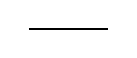
\begin{tikzpicture}
    \draw [thick] (0, 0) -- (1, 0); 
    \end{tikzpicture}
    & đường nét liền \\ \hline 

    %%%%%%%
    \begin{tikzpicture}
    \draw [very thick, dashed] (0, 0) -- (1, 0); 
    \end{tikzpicture}
    & đường nét đứt \\ \hline 

    %%%%%%%
    \begin{tikzpicture}
    \draw [very thick, dotted] (0, 0) -- (1, 0); 
    \end{tikzpicture}
    & đường nét chấm (đường chấm chấm)\\ \hline 

    %%%%%%%
    \begin{tikzpicture}
    \draw [very thick, dash pattern={on 7pt off 2pt on 1pt off 3pt}] (0,0) -- (1,0);
    \end{tikzpicture}
    & đường chấm gạch\\ \hline 
    %%%%%%%
    % \\[-3mm]
    % \vspace{1em}
    \begin{tikzpicture}[yshift = -1cm]
    \draw [pattern = dots] (0,0) rectangle (1,.4);
    \end{tikzpicture}
    & nền chấm\\\hline 
    %%%%%%%
    % \\[-1em]
    % \vspace{1em}
    \begin{tikzpicture}
    \draw [pattern = custom north west lines] (0,0) rectangle (1,.4);
    \end{tikzpicture}
    & nền sọc chéo\\ \hline 



    \end{tabular}
 \end{table} 




% Nhu cầu về nhân lực ngành Machine Learning (Deep Learning) đang ngày một cao, kéo theo đó nhu cầu học Machine Learning trên thế giới và ở Việt Nam ngày một lớn. Cá nhân tôi cũng muốn hệ thống lại kiến thức của mình về lĩnh vực này để chuẩn bị cho tương lai (đây là một trong những mục tiêu của tôi trong năm 2017). Tôi sẽ cố gắng đi từ những thuật toán cơ bản nhất của Machine Learning kèm theo các ví dụ và mã nguồn trong mỗi bài viết. Tôi sẽ viết 1-2 tuần 1 bài (việc viết các công thức toán và code trên blog thực sự tốn nhiều thời gian hơn tôi từng nghĩ). Đồng thơi, tôi cũng mong muốn nhận được phản hồi của bạn đọc để qua những thảo luận, tôi và các bạn có thể nắm bắt được các thuật toán này.

% Khi chuẩn bị các bài viết, tôi sẽ giả định rằng bạn đọc có một chút kiến thức về Đại Số Tuyến Tính (Linear Algebra), Xác Suât Thống Kê (Probability and Statistics) và có kinh nghiệm về lập trình Python. Nếu bạn chưa có nhiều kinh nghiệm về các lĩnh vực này, đừng quá lo lắng vì mỗi bài sẽ chỉ sử dụng một vài kỹ thuật cơ bản. Hãy để lại câu hỏi của bạn ở phần Comment bên dưới mỗi bài, tôi sẽ thảo luận thêm với các bạn.

% Trong bài tiếp theo của blog này, tôi sẽ giới thiệu về các nhóm thuật toán Machine Learning cơ bản. Mời các bạn theo dõi.

% \section{Tham khảo thêm}
% \subsection{Các khóa học}
% \subsubsection{Tiếng Anh}
% \begin{enumerate}
% 	\item \href{https://www.coursera.org/learn/machine-learning}{Machine Learning với thầy Andrew Ng trên Coursera} ({\it Khóa học nổi tiếng nhất về Machine Learning })

% 	\item \href{https://www.udacity.com/course/deep-learning -- ud730}{Deep Learning by Google trên Udacity} ({\it Khóa học nâng cao hơn về Deep Learning với Tensorflow})


% 	\item \href{http://machinelearningmastery.com/}{Machine Learning mastery} ({\it Các thuật toán Machine Learning cơ bản})
% \end{enumerate}

% \subsubsection{Tiếng Việt}
% {\bf Lưu ý}: {\it Các khóa học này tôi chưa từng tham gia, chỉ đưa ra để các bạn tham khảo.}
% \begin{enumerate}
% 	\item \href{http://tuanvannguyen.blogspot.com/2016/12/cap-nhat-khoa-hoc-ve-machine-learning.html}{Machine Learning 1/2017}


% 	\item \href{https://techmaster.vn/khoa-hoc/25511/machine-learning-co-ban}{Nhập môn Machine Learning, Tech Master- Cao Thanh Hà {\it POSTECH}}()

% \end{enumerate}

% \subsection{Các trang Machine Learning tiếng Việt khác}
% \begin{enumerate}
% 	\item \href{http://viet.jnlp.org/kien-thuc-co-ban-ve-xu-ly-ngon-ngu-tu-nhien/machine-learning-trong-nlp}{Machine Learning trong Xử Lý Ngôn Ngữ Tự Nhiên - Nhóm Đông Du {\it Nhật Bản}}

% 	\item \href{https://ongxuanhong.wordpress.com/}{Machine Learning cho người mới bắt đầu - Ông Xuân Hồng {\it JAIST}}.


% 	 \item \href{https://ml-book-vn.khanhxnguyen.com/}{Machine Learning book for Vietnamese - Nguyễn Xuân Khánh \textit{University of Maryland}}
% \end{enumerate}
% 3. [Machine Learning trong Xử Lý Ngôn Ngữ Tự Nhiên - Nhóm Đông Du _Nhật Bản_](http://viet.jnlp.org/kien-thuc-co-ban-ve-xu-ly-ngon-ngu-tu-nhien/machine-learning-trong-nlp)
% 4. [Machine Learning cho người mới bắt đầu - Ông Xuân Hồng _JAIST_](https://ongxuanhong.wordpress.com/).
% 5. [Machine Learning book for Vietnamese - Nguyễn Xuân Khánh _University of Maryland_](https://ml-book-vn.khanhxnguyen.com/)
